\clearpage



\begin{Indent}
  Fermi liquids are characterized by having $Z_{\bm k} > 0$ at the Fermi level!
\end{Indent}
It is a bit complicated to calculate~$\Sigma$ (see the integral expression in a previous chapter).
We will not perform the calculations here, but note that when the perturbation is the Coulomb potential, then the result is
\[
  \Sigma_I = -A_{\bm k}\, \mathrm{sgn}(\omega-\epsilon_F) (\omega-\epsilon_F)^2 = \Sigma_I(\bm k, \omega) \,,
\]
where $A_{\bm k} > 0$.
When $\omega \rightarrow \epsilon_F$, then $\Sigma_I \rightarrow 0$ as $(\omega-\epsilon_F)^2$:

\begin{figure}[H]
  \centering
  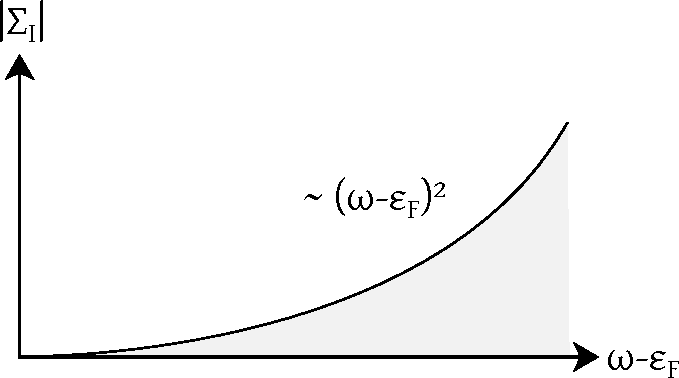
\includegraphics[width=0.5\textwidth]{img/pp181-200_selfenergy.pdf}
\end{figure}

The quasiparticles are well-defined close to the Fermi level because the damping is small.
If we get $\Sigma_I \sim (\omega-\epsilon_F)^2$, $\alpha < 1$, the damping disappears too slow, and $\alpha < 1$ is an indication that this is \emph{not} a Fermi liquid.
Finding a theoretical foundation for \emph{non}-Fermi liquid theory in $D>1$ dimensions is one of the big challenges in theoretical physics today (1995), since the normal ($T>T_c$) metallic state of high-$T_c$ superconductors exhibit transport properties that cannot be described as a Fermi liquid.
This may possibly be related to two-dimensional physics.

\emph{Heavy-fermion systems} (e.g. \ce{UPt3}): Correlation (Coulomb) effects are so large that the quasiparticles have masses $m^x/m \sim 1000$, and yet we have $Z_{k_F} > 0$!

3D: Fermi liquid theory is incredibly robust.

2D: ???

1D: Does not work, there is new physics here.



\clearpage
\section{Superconductivity}
\subsection{Introduction}
The perturbation theory we have considered so far is well equipped to describe \emph{quantitative} changes in e.g. electron systems caused by many-particle effects.
Pure perturbation theory is however not well suited to describe qualitative changes in a fermion or boson system caused by many-particle effects.
Examples of such qualitative changes may be:
\begin{enumerate}[(i)]
  \item Melting;
  \item Bose--Einstein condensation;
  \item Metal $\leftrightarrow$ insulator transitions;
  \item Metal/insulator  $\leftrightarrow$ superconductor transitions;
  \item Paramagnetic $\leftrightarrow$ ferromagnetic/antiferromagnetic transitions;
  \item Uniform electron gas $\leftrightarrow$ electron lattice (Wigner crystal) at low electron densities.
\end{enumerate}
Let $H = H_0 + V$, where $H_0$ for instance may describe a simple metal in in case~(iv) or a paramagnet in case~(v), and $V$ represents a perturbation that we expect to qualitatively change the ground state of $H_0$.

Absolutely \emph{all} transitions from one phase to another (i.e. phase transition)---such as e.g. the transition from a lattice to a fluid in the first example---are characterized by:

\begin{Indent}
  It is \emph{impossible} to reach one phase from a different phase by using a finite-order perturbation expansion in $V$.
\end{Indent}

If we wish to have any hope of describing transitions of type (i--vi) above, we need to do something different than pure perturbation theory.
We have already seen one example of this in problem set~1 (problem~2), where we replaced a many-particle problem by a selfconsistent one-particle problem that was exactly solvable.
In that case, we introduced a variational parameter~$\Delta$, which we determined by minimizing the energy with respect to~$\Delta$.
We will take a similar approach for the metal$\leftrightarrow$superconductor transition.
In problem set~1 (problem~2) the instability we considered was of type~(v), i.e. a transition from a non-magnetic to an antiferromagnetic state.
We saw that $\Delta\neq0$ signalized an \emph{ordering of spins}.
The model we considered was the Hubbard model,
\[
  H = \sum_{\langle i,j \rangle \sigma} t c^\dagger_{i\sigma} c_{j\sigma} + u\sum_i n_{i\uparrow} n_{i\downarrow} \,.
\]
We calculated non-perturbatively in $u$, and found that:
\[
  \Delta \sim e^{-1/Du} \,.
\]
NOTE: $\Delta$ is a non-analytic function of $u$.
This signalizes that the answer cannot be reached by any finite-order perturbation theory in $u$, because $\Delta$ is \emph{not} of the form
\[
  \Delta = \sum_{n=0}^\infty c_n u^n\,.
\]



\subsection{The Cooper Problem}
We have previously seen that it is possible for electrons to experience attractive interactions via phonons.
Before we attempt to solve this many-particle problem, we will first consider the consequences of electron--electron attraction in a much simpler model; the math will illustrate that the final result will not be attainable by a finite-order perturbation expansion in this case either.

The model we will use is as follows: Fermi sphere $\ket{\textrm{FS}}$ + two extra electrons at \emph{opposite sides} of $\ket{\textrm{FS}}$ with \emph{opposite spins}.
\begin{enumerate}[(i)]
  \item Electrons in $\ket{\textrm{FS}}$ do \emph{not} interact with each other;
  \item The extra electrons do not interact with $\ket{\textrm{FS}}$ except via the Pauli principle: $k>k_F$;
  \item The extra electrons are in the one-particle states $\ket{\bm k,\sigma}$ and $\ket{-\bm k,-\sigma}$;
  \item The two electrons interact attractively in a thin ``shell'' around the Fermi surface.
\end{enumerate}
\begin{figure}[H]
  \centering
  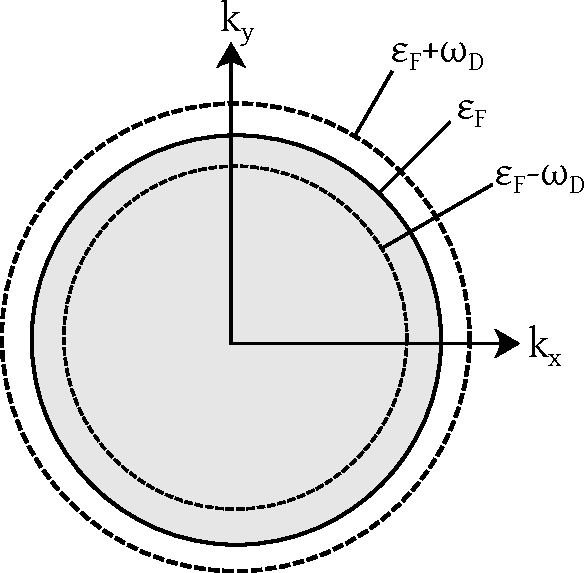
\includegraphics[width=0.5\textwidth]{img/pp181-200_fermisurface.pdf}
\end{figure}
The typical Debye frequency in a lattice is $\omega_D \sim 100$~K (since we assume a phonon-mediated attraction).

\clearpage
We will approximate the effective potential $\tilde{V}_\textrm{eff}$ by a step function:
\begin{figure}[H]
  \centering
  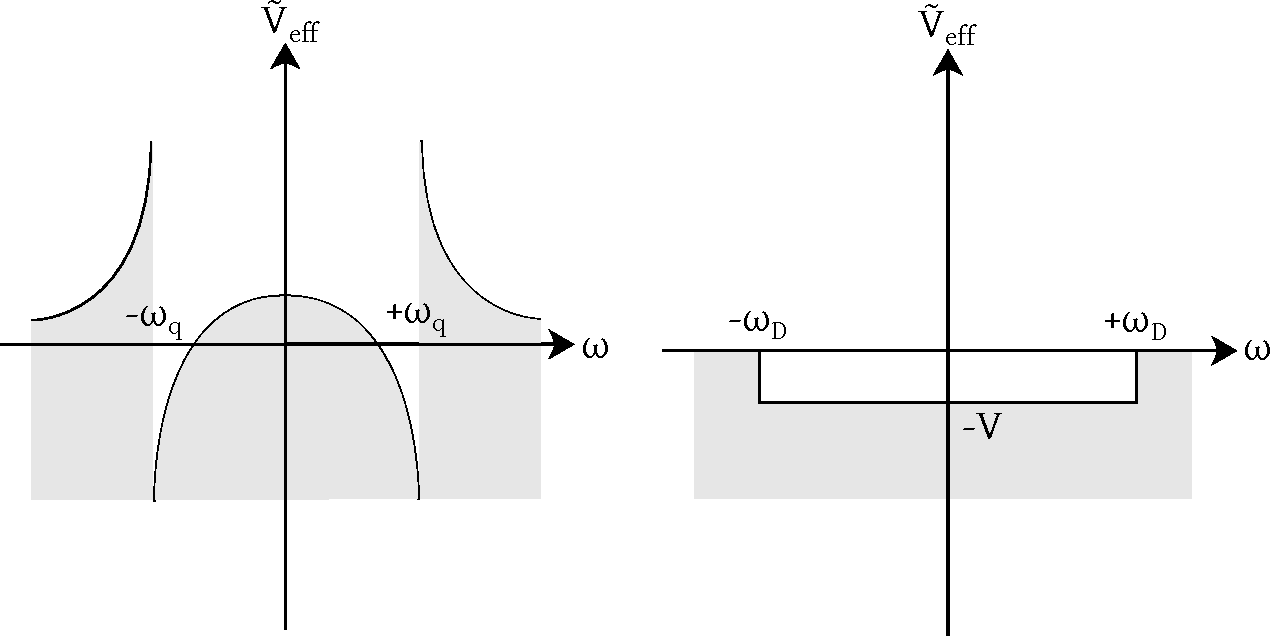
\includegraphics[width=\textwidth]{img/pp181-200_veffapprox.pdf}
\end{figure}
If at least one of the two electrons are outside of the thin shell around the Fermi level, they do not ``see'' each other.

We will solve this two-particle pproblem \emph{exactly}.
This will also provide a basis for discussing how well perturbation theory possibly could work.
\[
  H = H_0 + \tilde{V}_\textrm{eff}
\]
$H_0$: Kinetic energy of the two extra electrons.  \\
Exact two-particle state: $\ket{1,2}$. \\
If the electrons did not interact, then we would have the problem:
\[
  H_0 \ket{1,2}_0 = \epsilon_{\bm k} \ket{1,2}\,,
\]
which has the solution $\ket{1,2}_0 = \ket{\bm k,-\bm k}$.
$\epsilon_{\bm k}$: the \emph{kinetic} energy of the two extra electrons.

We now have to solve the problem:
\[
  (H_0 + \tilde{V}_\textrm{eff}) \ket{1,2} = E\ket{1,2} \,.
\]
From this Schrödinger equation we wish to find $\ket{1,2}$ and $E$.
$E$ is the energy of the \emph{interacting} two-electron system.

We start by expanding $\ket{1,2}$ in $\ket{1,2}_0 = \ket{\bm k,-\bm k}$:
\[
  \ket{1,2} = \sum_{\bm k'} a_{\bm k'} \ket{\bm k',-\bm k'}
\]
NOTE: $\bm k': \epsilon_{\bm k'} > 2\epsilon_F$ (Pauli principle, $\epsilon_{\bm k}$ two-electron energy) 

Substitute this into the Schrödinger equation:
\[
  \begin{aligned}
       \sum_{\bm k'} a_{\bm k'} \big[ H_0\ket{\bm k', -\bm k'} + \tilde{V}_\textrm{eff}\ket{\bm k', -\bm k'} \big]
    &= \sum_{\bm k'} Ea_{\bm k'} \ket{\bm k', -\bm k'} \big]  \\
    &\Downarrow \\
       \sum_{\bm k'} a_{\bm k'} \big[ E-\epsilon_{\bm k'} \big] \ket{\bm k', -\bm k'}  
    &= \sum_{\bm k'} a_{\bm k'} \tilde{V}_\textrm{eff}\ket{\bm k', -\bm k'} \big]
  \end{aligned}
\]
If we multiply by $\bra{\bm k,-\bm k}$ and use $\braket{\bm k,-\bm k|\bm k',-\bm k'} = \delta_{\bm k,\bm k'}$, we get an equation for determining $a_{\bm k}$ and $E$:
\[
  a_{\bm k}(\epsilon_{\bm k}-E) = -\sum_{\bm k'} a_{\bm k'} \braket{\bm k,-\bm k|\tilde{V}_\textrm{eff}|\bm k',-\bm k'} \equiv -\sum_{\bm k'} a_{\bm k'} V_{\bm k,\bm k'} \,,
\]
where the sum only extends over the values of $\bm k'$ that satisfy $\epsilon_{\bm k'} > 2\epsilon_F$.
The matrix element $V_{\bm k,\bm k'}$ describes the scattering process:
\begin{figure}[H]
  \centering
  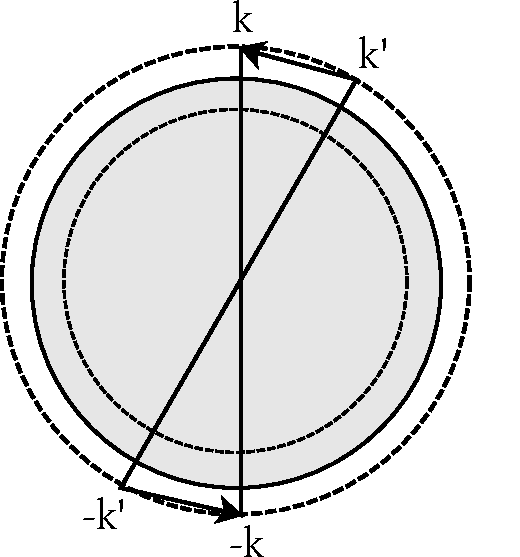
\includegraphics[width=0.45\textwidth]{img/pp181-200_coopermodel.pdf}
\end{figure}
\[
  V_{\bm k,\bm k'} =
  \begin{cases}
              -  V\,, & |\epsilon_{\bm k}-2\epsilon_F|, |\epsilon_{\bm k'}-2\epsilon_F|<2\omega_D\,; \\
     \phantom{-} 0\,, & \text{otherwise}.
  \end{cases}
\]
We then obtain
\[
  a_{\bm k}(\epsilon_{\bm k}-E) = V\sum_{\bm k'} \theta(2\omega_D - |\epsilon_{\bm k'} - 2\epsilon_F|) \,,
\]
and switch to an energy integration
\[
  a(\epsilon)(\epsilon-E) = V\int_{2\epsilon_F}^{2\epsilon_F+2\omega_D} \mathrm{d}\epsilon'\; a(\epsilon') N(\epsilon') \,,
\]
where $N(\epsilon')$ is the density of states.
We integrate over a thin shell around the Fermi level.
If we now assume that $N(\epsilon)$ varies slowly around the Fermi level, we may set $N(\epsilon) \approx N(2\epsilon_F)$.
We introduce $\lambda \equiv VN(2\epsilon_F)$:
\[
  a(\epsilon)(\epsilon-E) = \lambda \int_{2\epsilon_F}^{2\epsilon_F+2\omega_D} \mathrm{d}\epsilon'\; a(\epsilon') \,.
\]
The integral is independent of $\epsilon$!
This means that $a(\epsilon)(\epsilon-E) = \text{const}$, so:
\[
  a(\epsilon) = \frac{\text{const}}{\epsilon-E} \,.
\]
Thus, the expansion coefficients have been determined.

Now, what remains is to find the energy~$E$.
Substitute the ansatz $a(\epsilon) = \text{const}/(\epsilon-E)$ into the previous equation, 
\[
  \text{const} = \lambda \int_{2\epsilon_F}^{2\epsilon_F+2\omega_D} \mathrm{d}\epsilon'\; \frac{\text{const}}{\epsilon'-E} \,.
\]
This equation determines the eigenvalue $E$:
\[
  \frac{1}{\lambda} = \ln\left|\frac{2\epsilon_F+2\omega_D-E}{2\epsilon_F-E}\right|
\]
Introduce $\Delta \equiv 2\epsilon_F - E$, where $\Delta$ is the binding energy for the interacting two-electron system relative to free electrons at the Fermi level
\[
  \frac{1}{\lambda} = \ln\left(1+\frac{2\omega_D}{\Delta}\right) > 0 \,.
\]
Can only be solved if $\lambda > 0$: $V$ \emph{attractive}.
\[
  \Delta = 2\omega_D \frac{1}{e^{1/\lambda}-1}
\]
When $\lambda \ll 1$:
\[
  \Delta \approx 2\omega_D e^{-1/\lambda} \,.
\]

$\Delta$: Not an analytic function of $\lambda$.
Note the similarity with the answer from problem set~1, even if $\Delta$ now refers to something completely different.
\[
  \Delta \neq \sum_{n=0}^\infty b_n \lambda^n \,:
\]
We do not have any Taylor expansion in $\lambda$.
The form of the answer again indicates that binding between two electrons that are attracted to each other is a non-perturbative effect.

\begin{Indent}
  $\Delta>0 \Rightarrow$ bound state of two electrons $\ket{+\bm k,+\sigma}$ and $\ket{-\bm k,-\sigma}$. \\
  The bound state is called a \emph{Cooper pair}.
\end{Indent}

A few comments:
\begin{enumerate}[(i)]
  \item A Cooper pair is a paired state in $\bm k$-space, not in $\bm r$-space.
        Even if a ``hydrogen atom'' image of the Cooper pair some times can be useful, the $\bm r$-space analogy should not be taken too far.
  \item Even if we have explicitly calculated for only \emph{two} electrons, it is still hidden a kind of many-particle effect here via the Pauli principle.
        $\Delta \sim e^{-1/\lambda}$, $\lambda = 2VN\epsilon_F$. \\
        $\epsilon_k \sim k^2 \Rightarrow N(\epsilon) \sim \epsilon^{1/2}$ in $d=3$\\
        $\epsilon_F \rightarrow 0 \Rightarrow 2N\epsilon_F \rightarrow 0 \Rightarrow \lambda \rightarrow 0 \Rightarrow \Delta \rightarrow 0$\,.
        It is therefore necessary to have a Fermi sea in the problem to obtain the bound state.
        Two electrons in vacuum that interacted attractively would not form a Cooper pair.
  \item \emph{Quantum effect}: substitute back the Planck constant: $\Delta = 2\hbar \omega_D e^{1\lambda}$. 
        In the classical limit $\hbar \rightarrow 0$, we also get $\Delta \rightarrow 0$.
        A classical electron gas with attractive interactions do not yield Cooper pairs.
        Can never explain Cooper pairs from Newtons equations.
  \item \emph{Temperature effect}: If we increase $T$, we will get thermal dissociation of Cooper pairs.
        We expect that all pairs are dissociated at a temperature such that $T \sim \Delta$.
\end{enumerate}





\clearpage
\subsection{The Bardeen--Cooper--Schrieffer Theory of Superconductivity}
The theory needs to explain:
\begin{enumerate}[(i)]
  \item Zero electrical resistivity below a certain critical temperature $T_c$;
  \item \emph{Meissner effect}: magnetic fields are ``expelled'' from a superconductor below the critical temperature~$T_c$, when the metal is cooled down in \emph{zero} external magnetic field.
        The superconductor has a \emph{perfect} diamagnetic response.
\end{enumerate}
An important observation was that the critical temperature varied with the ionic mass of the lattice (something that could be observed by isotope substitution).
In other words, the critical temperature has an \emph{isotope effect}.
This indicates that phonons are important for the problem.
When we will write down a Hamiltonian that contains the right physics, it is therefore natural to include electron--phonon--electron interactions.
We have considered:
\[
  H = \sum_{\bm k,\sigma} \epsilon_{\bm k} c^\dagger_{\bm k,\sigma} c^{\phantom{\dagger}}_{\bm k,\sigma}
    + \sum_{\bm k,\sigma} \sum_{\bm k',\sigma'}\sum_{\bm q} \tilde{V}_\textrm{eff} c^\dagger_{\bm k+\bm q,\sigma} c^\dagger_{\bm k'-\bm q,\sigma'} c^{\phantom{\dagger}}_{\bm k',\sigma'} c^{\phantom{\dagger}}_{\bm k,\sigma}
\]
This is the standard form for second-quantized interacting electron gas in the planewave basis
\[
  \tilde{V}_\textrm{eff} = \frac{|M_{\bm q}|^2}{\omega^2-\omega^2_{\bm q}} + \frac{4\pi e^2}{\bm q^2}
\]
$M_{\bm q}$: electron--phonon coupling.
Energy transfer $\omega$:
\[
  \omega = \epsilon_{\bm k'} - \epsilon_{\bm k} = \epsilon_{\bm k'-\bm q} - \epsilon_{\bm k + \bm q} = \epsilon_{\bm k+\bm q} - \epsilon_{\bm k} = \epsilon_{\bm k'-\bm q} - \epsilon_{\bm k'}
\]
For now, forget about the Coulomb interactions.
We may for instance assume that the Coulomb potential is screened:
\[
  \tilde{V}_\textrm{eff} = \frac{|M_{\bm q}|^2}{(\epsilon_{\bm k}-\epsilon_{\bm k+\bm q})^2 - \omega_{\bm q}^2} = \tilde{V}_\textrm{eff}(\bm k,\bm q)
\]
$\tilde{V}_\textrm{eff} < 0$ for \emph{all} $\bm k, \bm k', \bm k+\bm q, \bm k'-\bm q$ such that:
\[
  \begin{aligned}
    |\epsilon_{\bm k}  - \epsilon_{\bm k+\bm q}|  &< \omega_{\bm q} \,, \\
    |\epsilon_{\bm k'} - \epsilon_{\bm k'-\bm q}| &< \omega_{\bm q} \,, 
  \end{aligned}
\]
From here on, we will focus on the scattering processes that lead to attraction between electrons.
The processes that lead to repulsion are not expected to do anything that the Coloumb potential isn't doing already, which in good metals is essentially \emph{nothing}.
With this goal in mind, we will simplify the Hamiltonian.

\emph{First simplification}:
What $\bm k,\bm k',\bm q$ give the main contributions to the Hamiltonian such that $\tilde{V}_\text{eff} < 0$?
$\epsilon_{\bm k}, \epsilon_{\bm k+\bm q}, \epsilon_{\bm k'}, \epsilon_{\bm k'-\bm q}$ must \emph{all} lie in a thin shell around the Fermi level.
$\bm k, \bm k'$ must stay within a thin shell.
This forces $\bm k'-\bm q$ and $\bm k+q$ to do the same!
\begin{figure}[H]
  \centering
  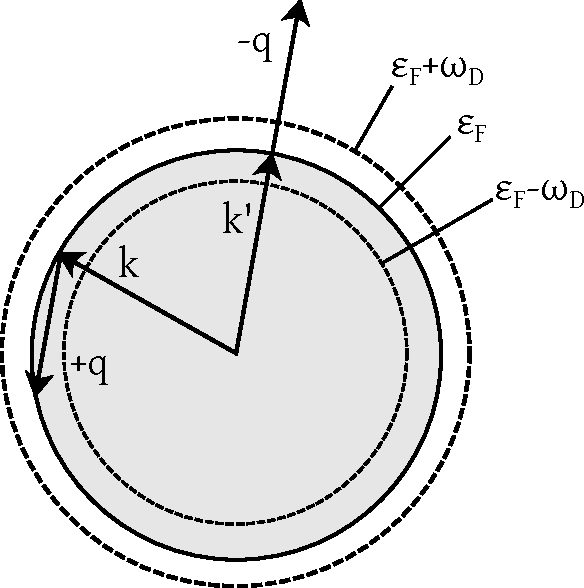
\includegraphics[width=0.5\textwidth]{img/pp181-200_cooperlimits.pdf}
\end{figure}
As we see, this places severe limitations on $\bm q$: even if $\bm k+\bm q$ lies within the shell, $\bm k'-\bm q$ does not have to do the same.
But: there is \emph{one} case, where any $\bm q$ such that $\bm k+\bm q$ lies within a thin shell, \emph{also} causes $\bm k'-\bm q$ to do the same: when $\bm k'=\bm -k$.
$\bm q$ is the momentum transferred in the scattering process.
If $\bm k'=-\bm k$, this would maximize the number of allowed ascattering processes around the Fermi level.
We assume that terms such that $\bm k'=-\bm k$ will therefore dominate the Hamiltonian completely, so \emph{we will only include such terms}.

\emph{Second simplification}:
We will only include terms where $\sigma'=-\sigma$.
If the interaction is short-ranged (of the type in the Hubbard model: ``on-site''), this would be natural.

Thus we obtain the simplified model:
\[
  H = \sum_{\bm k,\sigma} \epsilon_{\bm k} c^\dagger_{\bm k,\sigma} c^{\phantom{\dagger}}_{\bm k,\sigma}
    + \sum_{\bm k,\bm k'} V_{\bm k,\bm k'} c^\dagger_{\bm k,\uparrow} c^\dagger_{-\bm k,\downarrow} c^{\phantom{\dagger}}_{-\bm k',\downarrow} c^{\phantom{\dagger}}_{\bm k',\uparrow}
\]
\emph{This is the BCS model of a superconductor}.
It describes electrons with a special kind of interactions, which are such that the electrons in state $\ket{\bm k,\uparrow}$ and $\ket{-\bm k,\downarrow}$ around the Fermi level are those that interact attractively.
Other electrons will essentially just not notice each other.
Note that in the second term, $\bm k,\bm k'$ are within a thin shell around the Fermi surface.

